\documentclass[10pt]{article}
\usepackage{multicol}
\usepackage[a4paper, margin=2cm]{geometry}
\usepackage{float}
\usepackage{graphicx}
\graphicspath{ {./images/} }
\usepackage[colorlinks=true,linkcolor=blue]{hyperref}%
\usepackage{microtype} 			% para melhorias de justificação
\usepackage[backend=biber]{biblatex}
\usepackage{newclude}
\addbibresource{refs.bib}


\author{João Pedro Miranda Marques - 2017050495}

\begin{document}

\begin{titlepage}
    \begin{center}
           
    {\large Universidade Federal de Minas Gerais\\
    Escola de Engenharia \\
    Curso de Graduação em Engenharia de Controle e Automação\\}
    \vfill

    \begin{figure}[h]
        \centering
        
\includegraphics[scale=0.5]{images/brasao_ufmg.png}
    \end{figure}
    \vspace{2cm}


    {\bf\Large EHDA closed loop control system based on real time non-visual spray mode classification\\}
    \vspace{1cm} 
    {\Large Relatório de Atividades 3   \\  Projeto Final de Curso}
    \vspace{2cm}  
    
    %\hspace{0.3\textwidth} 
    {\large Orientador: Vitor Angelo\\
            Supervisor: Luewton L F Agostinho}\\

    
    %\hspace{0.3\textwidth} \parbox{0.65\textwidth}
    {\large Aluno: João Pedro Miranda Marques \\
    Matricula: 2017050495}
    \vspace{2cm}  

    \today
    \vspace{2cm}  
       

    %\hspace{0.3\textwidth} 
    \large \date{\today}
    \end{center}
    
    \end{titlepage}
    
    \newpage
    \clearpage
    \thispagestyle{empty}
    
    \cleardoublepage


\title{
    EHDA closed loop control system based on real time non-visual spray mode classification \\
    \large Relatório de Atividades}



Electrohydrodynamic Atomization (EHDA), also known as Electrospray (ES), is a way to disintegrate a liquid into droplets by exposing it to a strong electric field.
The electric current flowing transported by the spray reveals characteristic shapes for different spray modes.
Signal processing techniques can allow a non-visual classification of the spray mode based on the electric current shape.
The spray process imposes noise and random sequences on the measured signal making its classification not a trivial task. 
Industrial applications demand automated stabilization of a spray mode.
This can be achieved by a closed-loop control system. This project is about to develop an application that can classify what dynamics the EHDA experiment is current in and control
the variables to stabilize in the desired mode. In the figure we can see how EHDA experiment works.

\begin{figure}[H]
    \center
    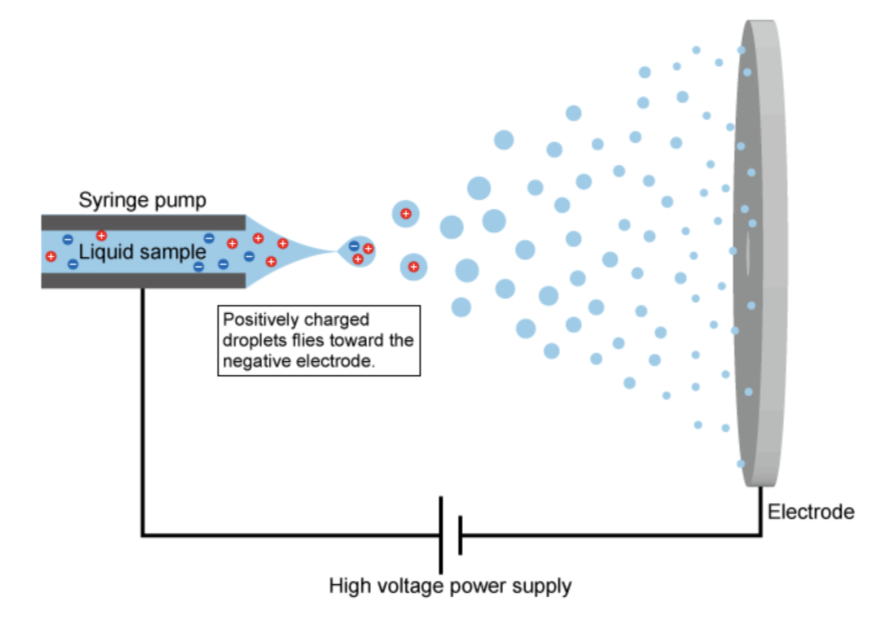
\includegraphics[width=8cm]{images/electrospray.png}
    \label{img1}
    \caption{EHDA example}
\end{figure}

This project was inspired by the research \emph{A generic electrospray classification} \cite*[]{Sjaaks}.
In this paper the author studied the current signal through the high voltage circuit in the EHDA experiment.
This signal is highly correlated with the spraying dynamics because the current is flowing with the liquid charges sprayed.
The author analysed this current data grouping samples in a time window. With observation in the data and the process he could
notice that the dynamic mode of the spray can be classified using statistical measurements of the signal. In his research the author 
emphasised the separability in the data using the relations between mean, median and standart deviation of the signal. This paper is important
for this project because the author explored the classification with non visual data. By the other side, the author focused his research in statistical values
in the time domain. In the project we can explore more the data characteristics in the frequency domain.

Another project is the \emph{experimental investigation of scaling laws for electrospraying: dieletric constant effect}\cite*[]{Chen_Pui}.
Where the author study about the quemical properties of the liquid being sprayed that can actually interfere in the dynamics of the process. 
In the paper the author emphasised about the liquid dieletric constant. For us this paper is interesting because we can understand better which liquid
has a better margin of operation in cone jet mode for example. What is missing in his article is that it is not mentioning all the variables that can interfere in the 
electrospray dynamics, which would be important to know.



\pagebreak
\printbibliography
\end{document}



